\documentclass[a4paper]{article}
\usepackage[utf8]{inputenc}
\usepackage[T1]{fontenc}
\usepackage[spanish]{babel}
\usepackage{lmodern}
\usepackage[margin=2cm, top=2cm, includefoot]{geometry}
\usepackage{graphicx}
\usepackage{xcolor}
\usepackage{fancyhdr}
\usepackage[most]{tcolorbox}
\usepackage[hidelinks]{hyperref}
\usepackage{parskip}
\usepackage{smartdiagram}
\usepackage{listings}
\usepackage{zed-csp}
\title{Práctica}
\author{José Rodolfo}
\date{\today}
\definecolor{greenPortada}{HTML}{69A84F}
\definecolor{codegreen}{rgb}{0,0.6,0}
\definecolor{codegray}{rgb}{0.5,0.5,0.5}
\definecolor{codepurple}{rgb}{0.58,0,0.82}
\definecolor{backcolour}{rgb}{0.95,0.95,0.92}
\newcommand{\vbMachineName}{Mario}
\newcommand{\vbHTBLogo}{img/htb-logo-2.png}
\newcommand{\vbMarioLogo}{img/mario.png}
\newcommand{\startDate}{21 de Marzo del 2020}
\pagestyle{fancy}
\fancyhf{}
\setlength{\headheight}{1.5cm}
\lhead{\includegraphics[width=0.25\textwidth]{\vbHTBLogo}}
\rhead{\includegraphics[height=1.5cm]{\vbMarioLogo}}
\cfoot{\thepage}
\renewcommand{\headrulewidth}{3pt}
\let\oldheadrule\headrule
\renewcommand{\headrule}{\color{greenPortada}\oldheadrule}
\lstdefinestyle{mystyle}{
    backgroundcolor=\color{backcolour},
    commentstyle=\color{codegreen},
    keywordstyle=\color{magenta},
    numberstyle=\tiny\color{codegray},
    stringstyle=\color{codepurple},
    basicstyle=\ttfamily\footnotesize,
    breakatwhitespace=false,
    breaklines=true,
    captionpos=b,
    keepspaces=true,
    numbers=left,
    numbersep=5pt,
    showspaces=false,
    showstringspaces=false,
    showtabs=false,
    tabsize=2
}
\lstset{style=mystyle}
\renewcommand{\lstlistingname}{Código}
\begin{document}
  \begin{titlepage}
    \centering
    \includegraphics[width=0.75\textwidth]{\vbHTBLogo}\par
    {\scshape\LARGE\textbf{Informe Técnico}}\par
    \vspace{5mm}
    {\Huge\bfseries\textcolor{greenPortada}{Máquina \vbMachineName}}\par
    \vfill
    \includegraphics[height=0.75\textwidth]{\vbMarioLogo}\par
    \vfill
    \begin{tcolorbox}[colback=red!5!white,colframe=red!75!black]
      \centering
      Este documento es confidencial y contiene información sensible.\\
      No deberia ser impreso o compartido con terceras entidades.
    \end{tcolorbox}
    {\large\startDate}
  \end{titlepage}
  \newpage
  \renewcommand{\contentsname}{Tabla de contenido}
  \tableofcontents
  \newpage
  \section{Antecedentes}
  El presente documento contiene los resultados obtenidos durante la fase de auditoria realizada a al máquina \vbMachineName de la plataforma \href{https://hackthebox.eu/}{\textbf{\color{greenPortada}HackTheBox}}.
  \begin{figure}[h]
    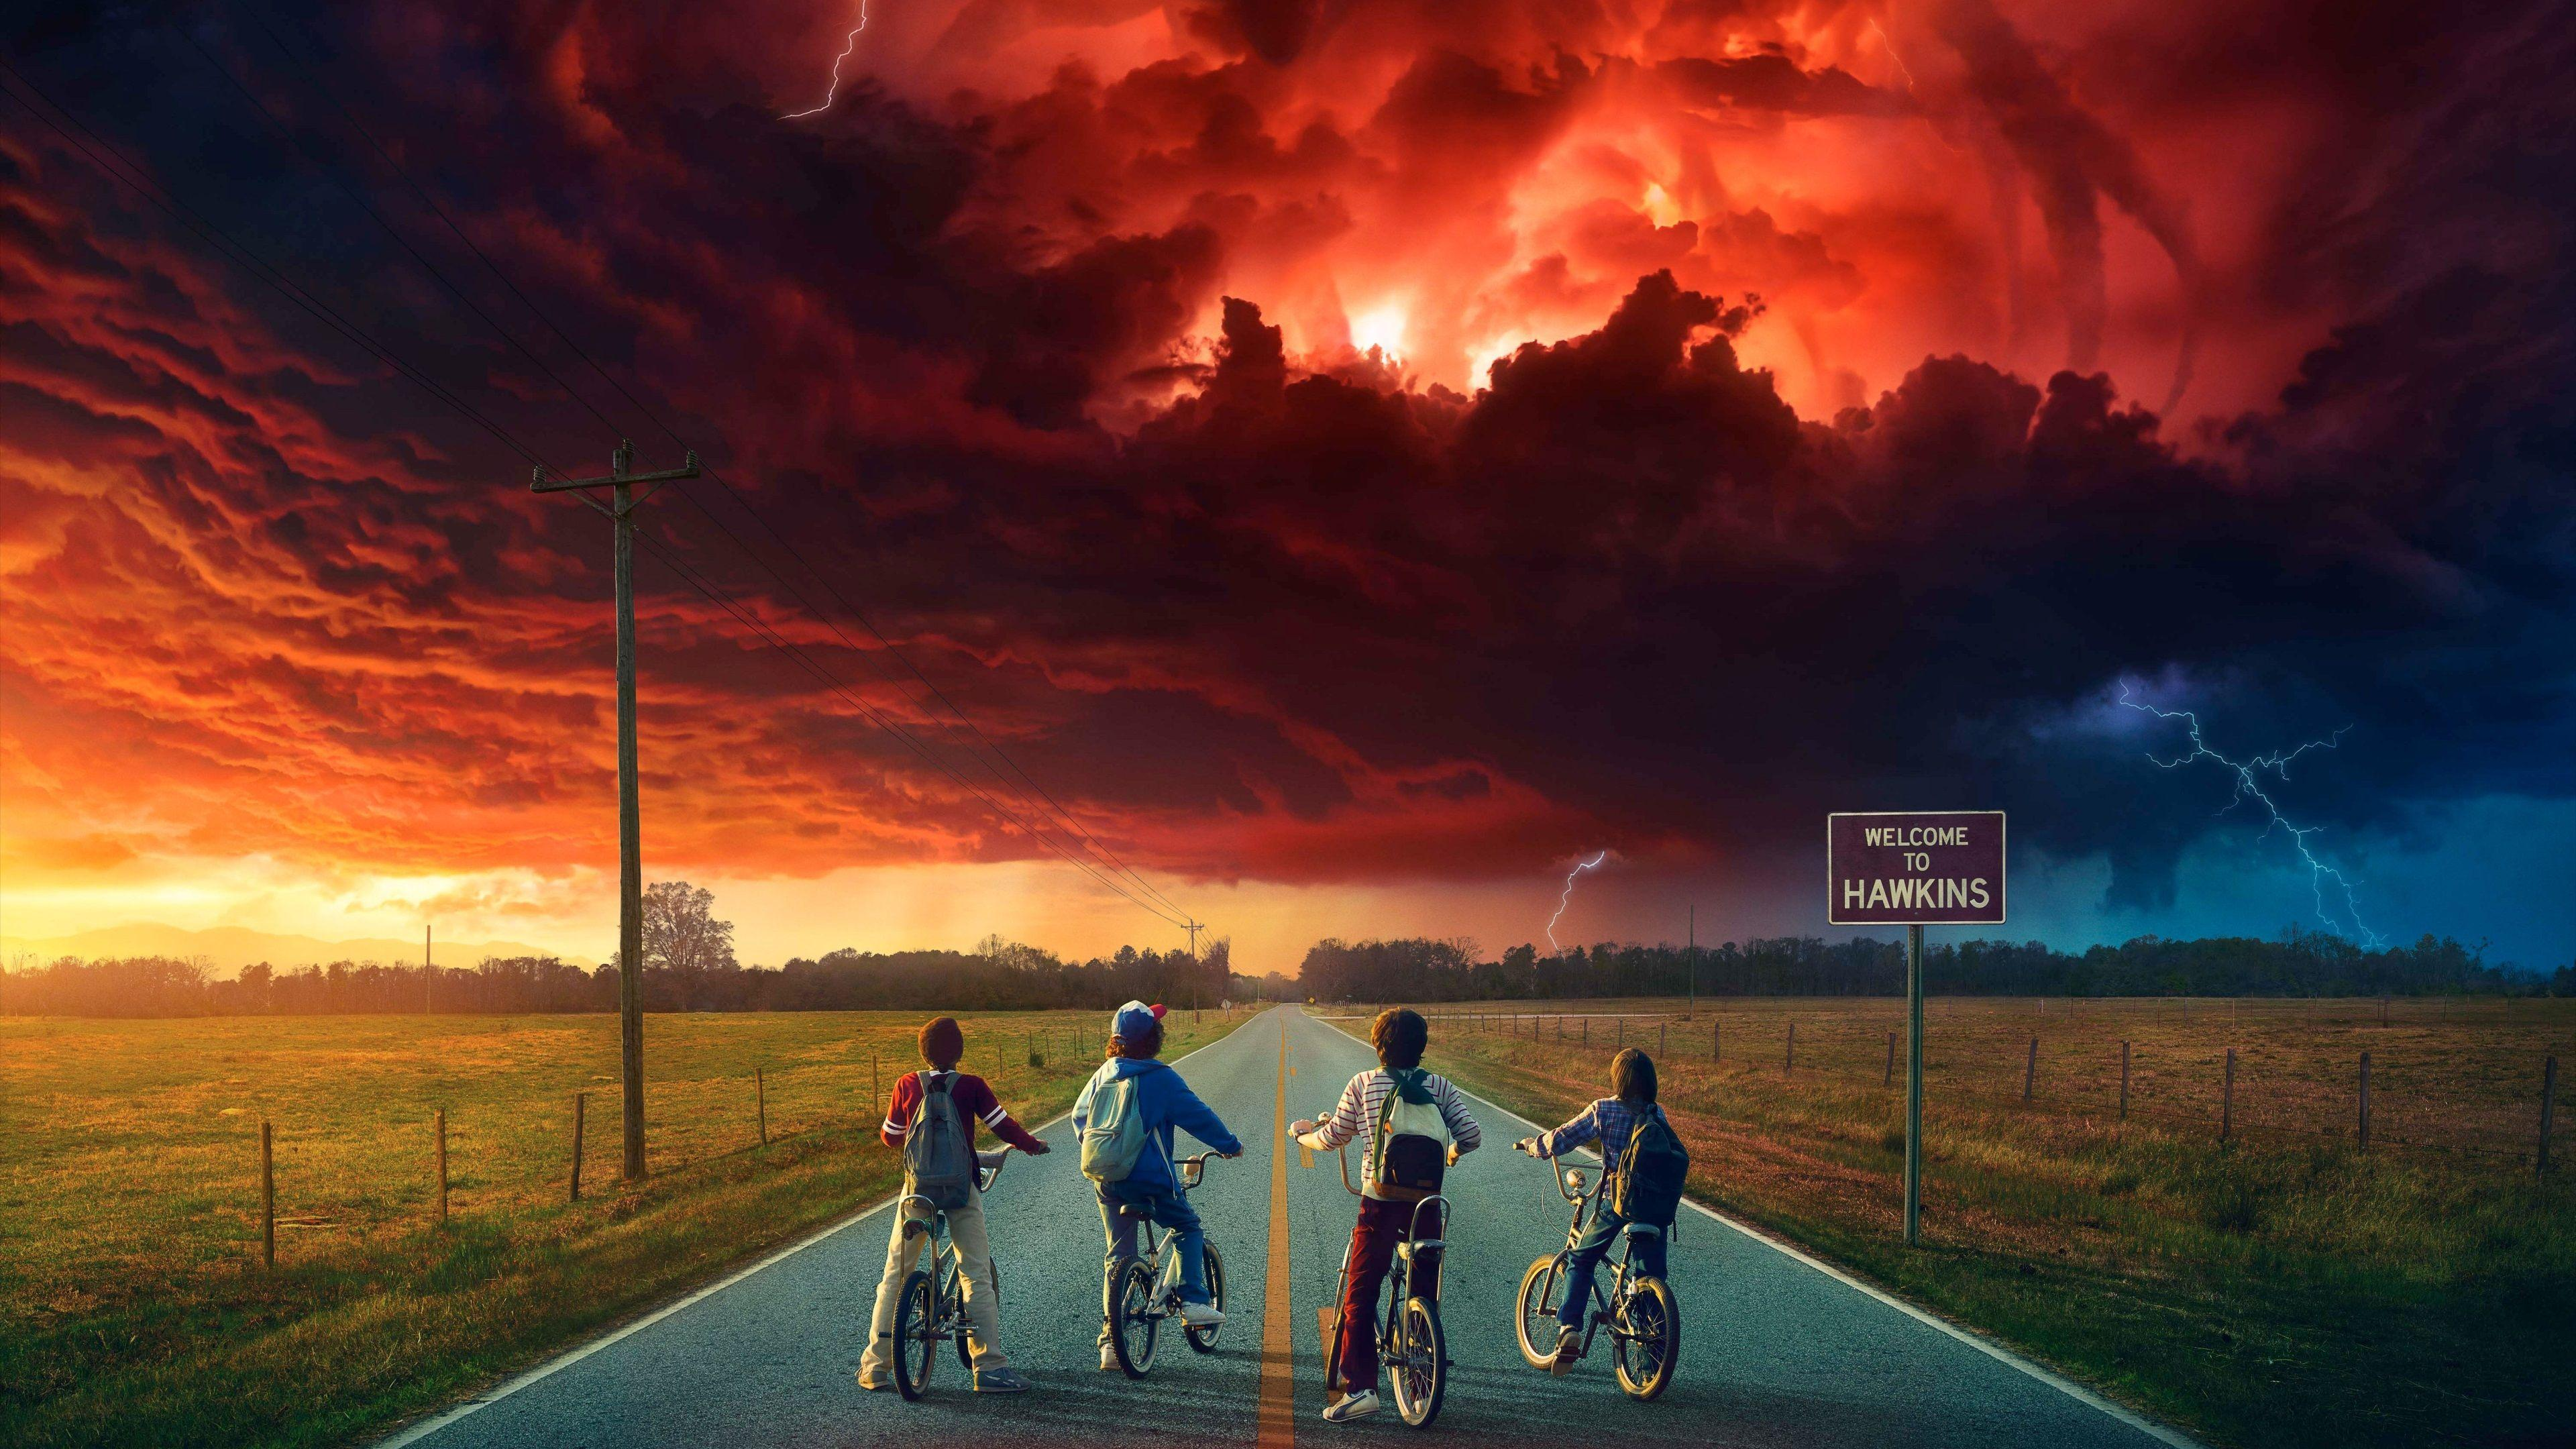
\includegraphics[width=\textwidth]{img/stranger-things.jpg}
    \caption{Datos de la Máquina \vbMachineName}
  \end{figure}
  \section{Objetivos}
  Conocer el estado de seguridad actual del servidor \textbf{\vbMachineName}, enumerando posibles vectores de explotación y determinando el alcance e impacto que un atacante podría ocasionar sobre el sistema en producción.
  \subsection{Consideraciones}
  Una ves finalizadas las jornadas de auditoria, se llevará a cabo una fase de saneamiento y buenas prácticas con el objetivo de securizar el servidor y evitar ser víctimas de un futuro ataque en base a los vectores explotados.
  \begin{figure}[h]
    \begin{center}
      \smartdiagram[priority descriptive diagram]{
        Reconocimiento sobre el sistema,
        Detección de vulnerabilidades,
        Explotación de vulnerabilidades,
        Securización del sistema
      }
    \end{center}
    \caption{Flujo de trabajo}
  \end{figure}
  \newpage
  \section{Análisis de vulnerabilidades}
  \subsection{Reconocimiento inicial}
  Se comenzó realizando un análisis inicial del sistema, verificando que el sistema objetivo se encontrara accesible desde el segmento de red en el que se opera:\par
  \begin{figure}[h]
    \begin{center}
      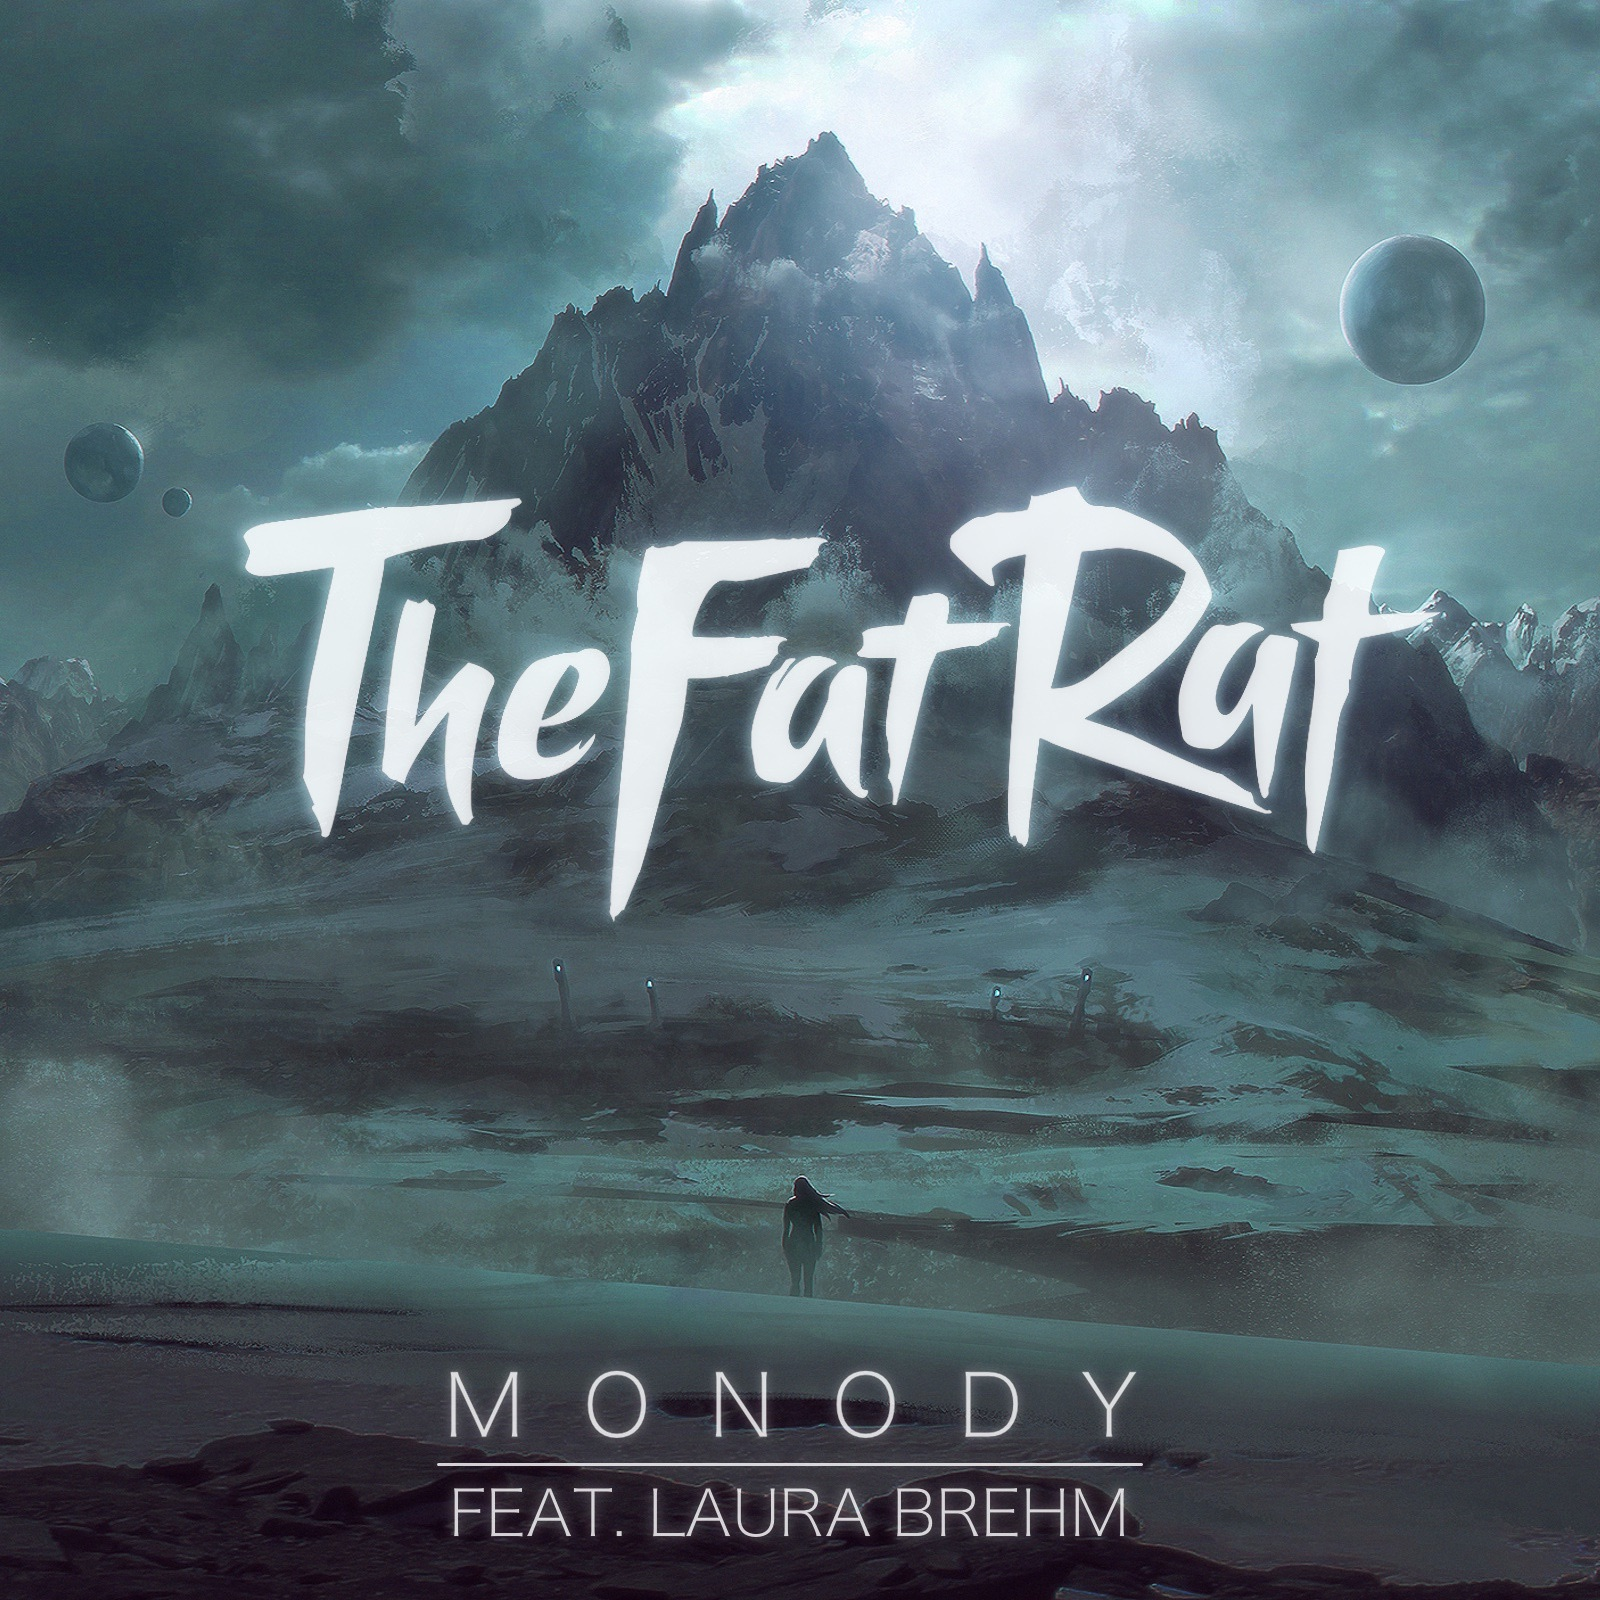
\includegraphics[width=0.5\textwidth]{img/thefatrat-ft.laura-brehm-monody.jpg}
    \end{center}
    \caption{Reconocimiento inicial sobre el sistema objetivo}
  \end{figure}
  Una vez localizado, se realizó un escaneo a través de la herramienta \textbf{nmap} para la detección de puertos abiertos, obteniendo los siguientes resultados:
  \begin{figure}[h]
    \begin{center}
      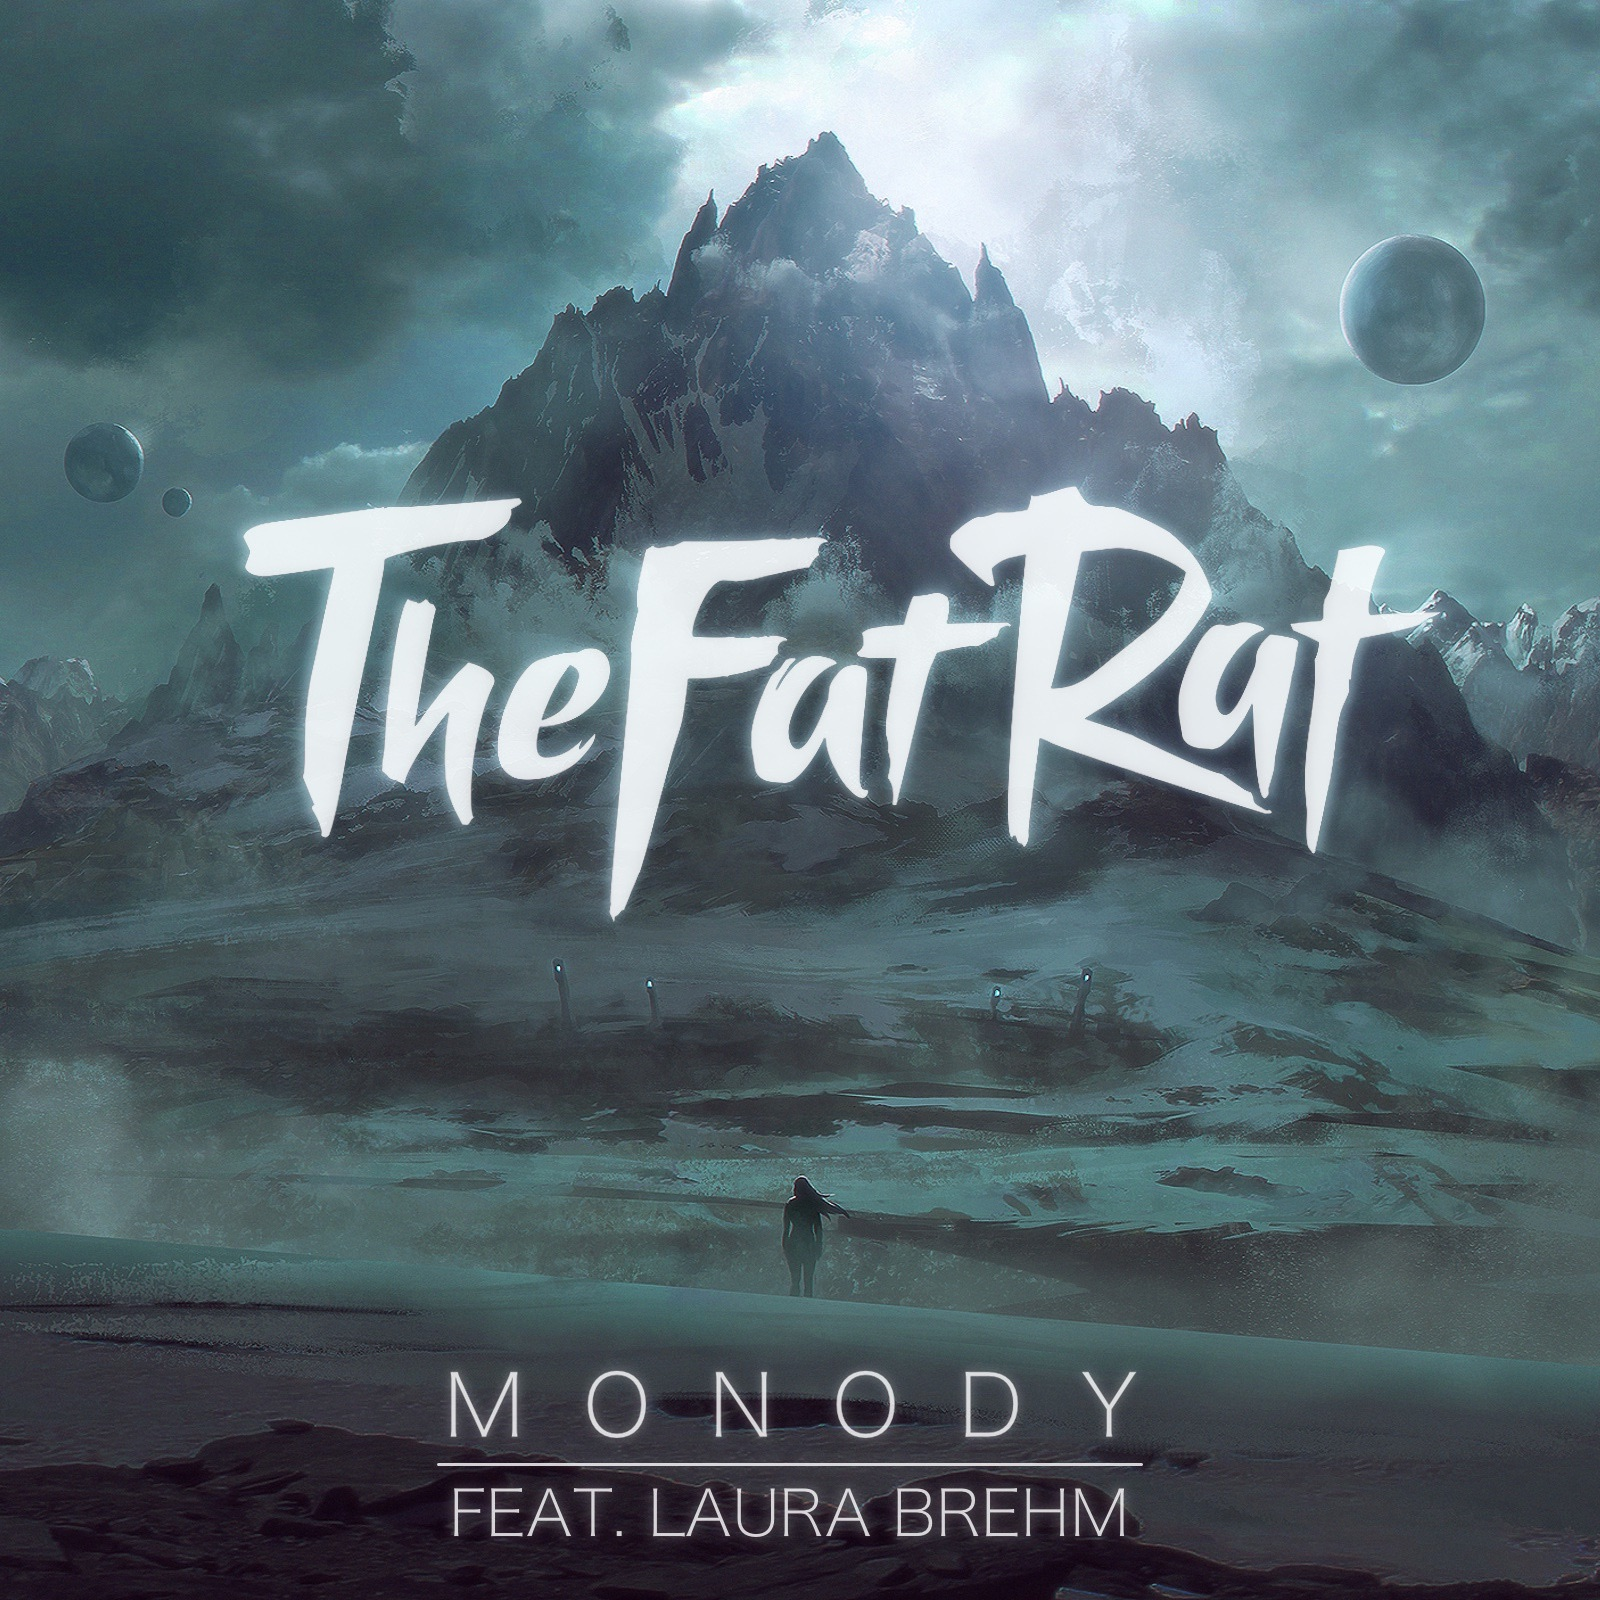
\includegraphics[width=0.5\textwidth]{img/thefatrat-ft.laura-brehm-monody.jpg}
    \end{center}
    \caption{Reconocimiento con nmap}
  \end{figure}
  \newpage
  Asimismo, con el objetivo de evitar falsos positivos, se diseño un script en \textbf{Bash} para enumerar posible puertos adicionales que la herramienta nmap no llegara a detectar.\par
  \begin{lstlisting}[language=Bash, caption=Script personalizado para enumerar puertos]
  #!/bin/bash
  for port in $(seq 1 65535); do
    timeout 1 bash -c "echo > /dev/tcp/10.10.10.52/$port" > /dev/null 2>&1 && echo "$port/tcp" &
  done; wait
  \end{lstlisting}
  A través de este script, fue posible detectar puertos adicionalmente abiertos:
  \begin{schema}{TCP}
    Puertos
    \where
    593, 1337
  \end{schema}
  Una vez finalizada la fase de enumeración de puertos, se detectaron los servicios y versiones que corrían bajo estos, representando a continuación los más significativos bajo los cuales fue posible explotar el sistema:\par
  \begin{figure}[h]
    \centering
    \makebox[\textwidth]{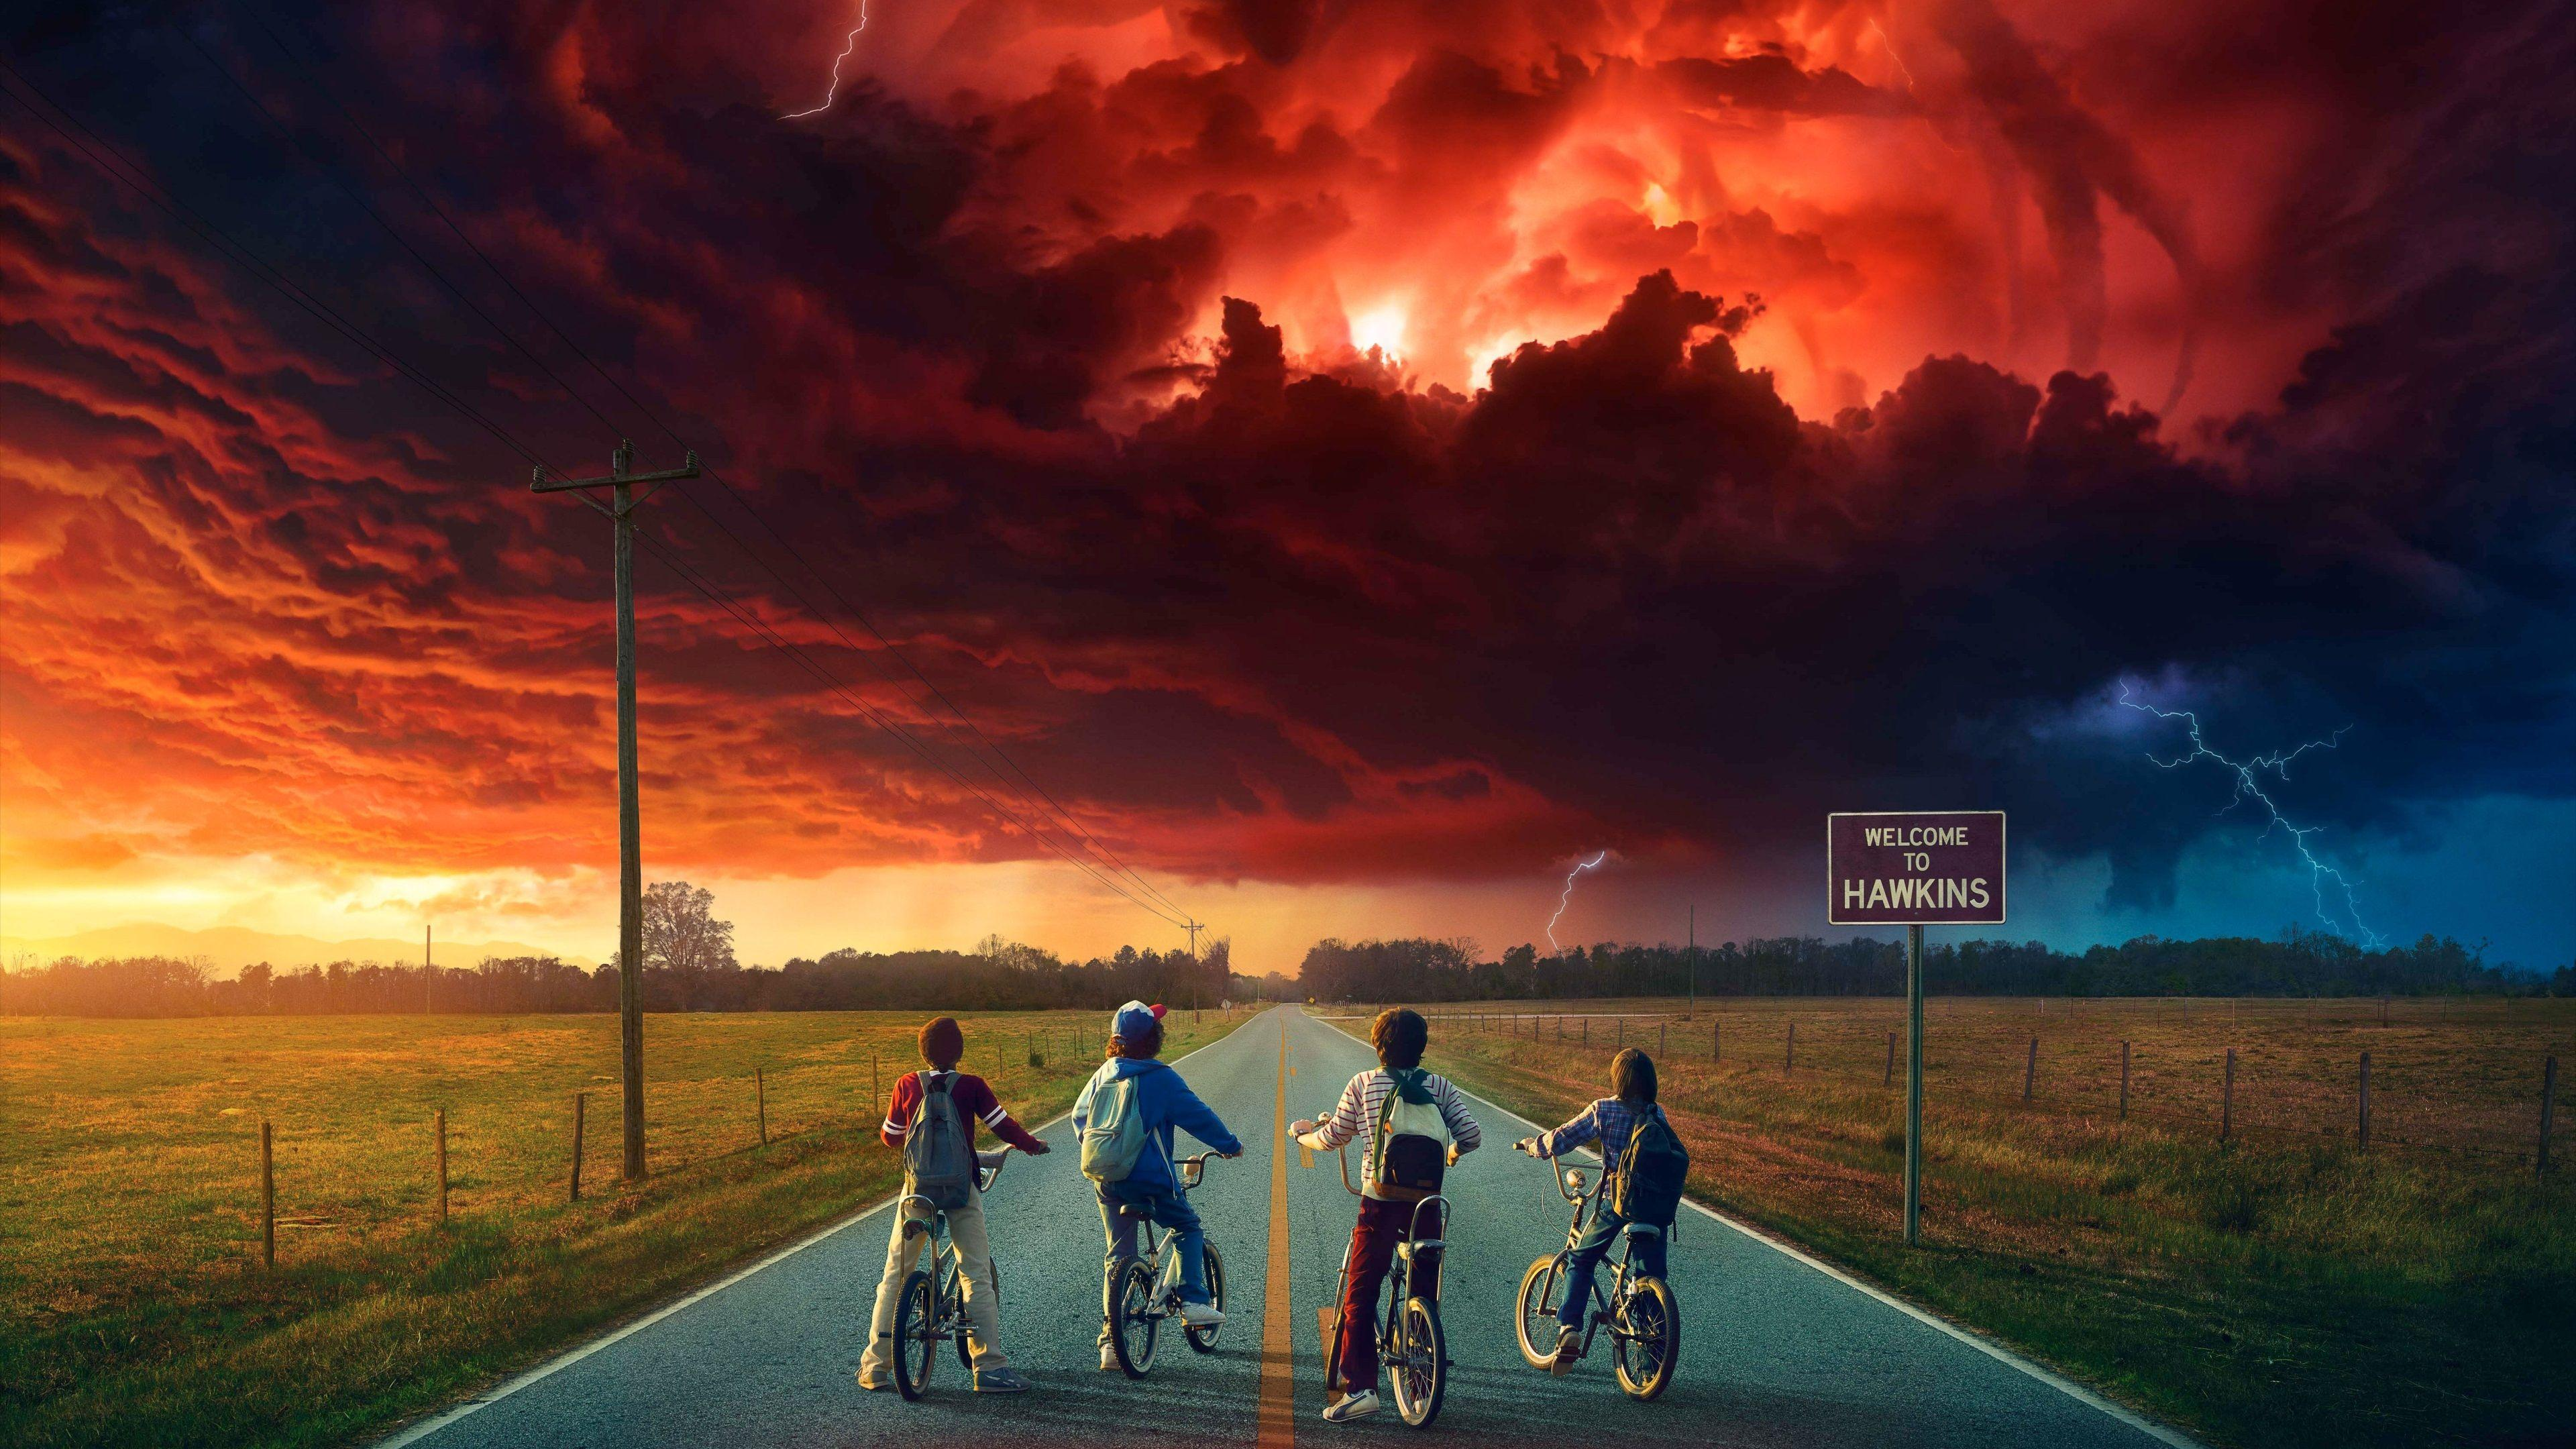
\includegraphics[width=0.9\paperwidth]{img/stranger-things.jpg}}
    \caption{Enumeración de servicios y versiones}
    \label{fig:servicesResults}
  \end{figure}
  Tal y como se aprecia en la figura ~\ref{fig:servicesResults}
\end{document}